%\mychapter{6}{Results}

\section{Results}
In this section, we report results on  synthetic data using diffusion maps. We compare our results with those obtained via PCA, a popular linear dimensionality technique. We apply PCA and diffusion maps to both the 
clean firing rate data set and the spike time data set preprocessed  with the previous time measure to obtain previous time data (see Figure \ref{fig:Simulated_datasets}).\\

Figure \ref{fig:DiffMaps_PCA_on_Prevtime_FR} (left column) shows that both diffusion maps  and PCA capture the animal's motion around the circular track when applied on firing rate data. This is not surprising since we are using clean firing rate data that encodes the animal's position around the track. However, when using previous time data, diffusion maps  appears to outperform PCA (see the right column of Figure  \ref{fig:DiffMaps_PCA_on_Prevtime_FR}). We  see that analyzing previous time data using diffusion maps captures the simulated four and half laps taken by the animal around the circular track while PCA  fails to reveal that the rat took four and a half laps  around the track. 
In otherwords, only diffusion maps  reveals the structure of a one-dimensional  manifold expected from the fact that 
the neural activity is strongly correlated with the rat's position.

\begin{figure}[H]
        \centering
        \begin{subfigure}[b]{0.475\textwidth}
            \centering
            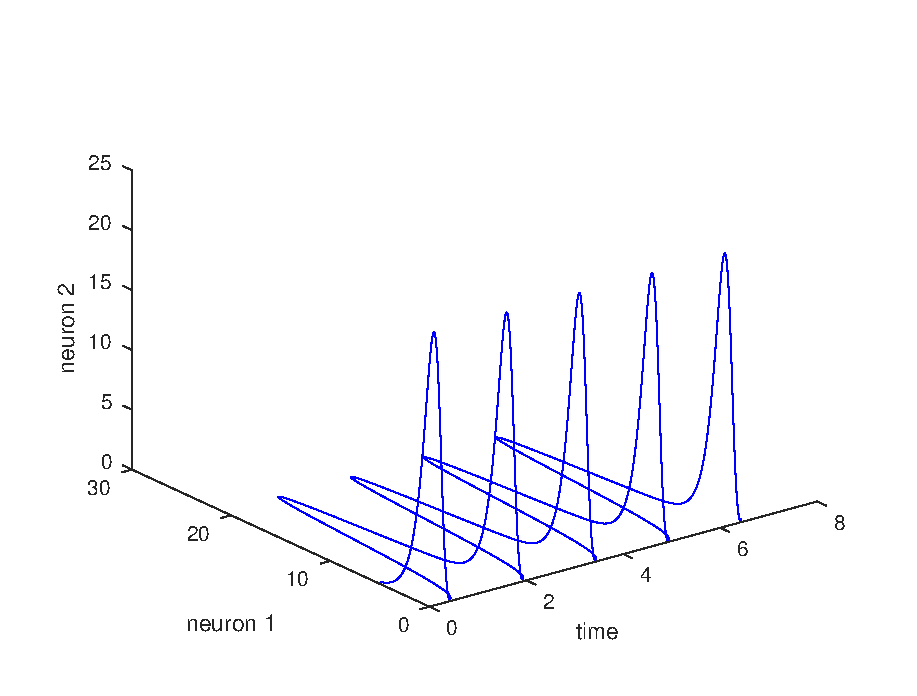
\includegraphics[width=\textwidth]{./images/SimFiringRate-with-time.eps}
           % 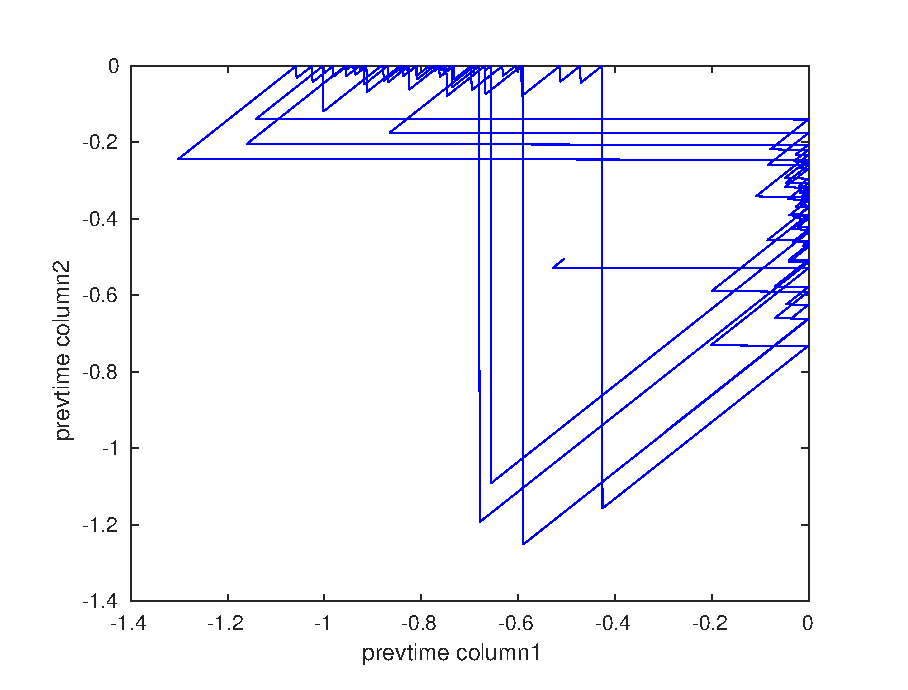
\includegraphics[width=\textwidth]{./images/FinalOralPlots/SyntheticOralPaper/SimPrevtime.eps}
            \caption[]%
            {{\small Simulated firing rate data (FR)}}  
            %{{\small Simulated previous time data (Prevtime)}} 
               
            \label{fig:Prevtime in 3D}
        \end{subfigure}
        \hfill
        \begin{subfigure}[b]{0.475\textwidth}  
            \centering 
           % 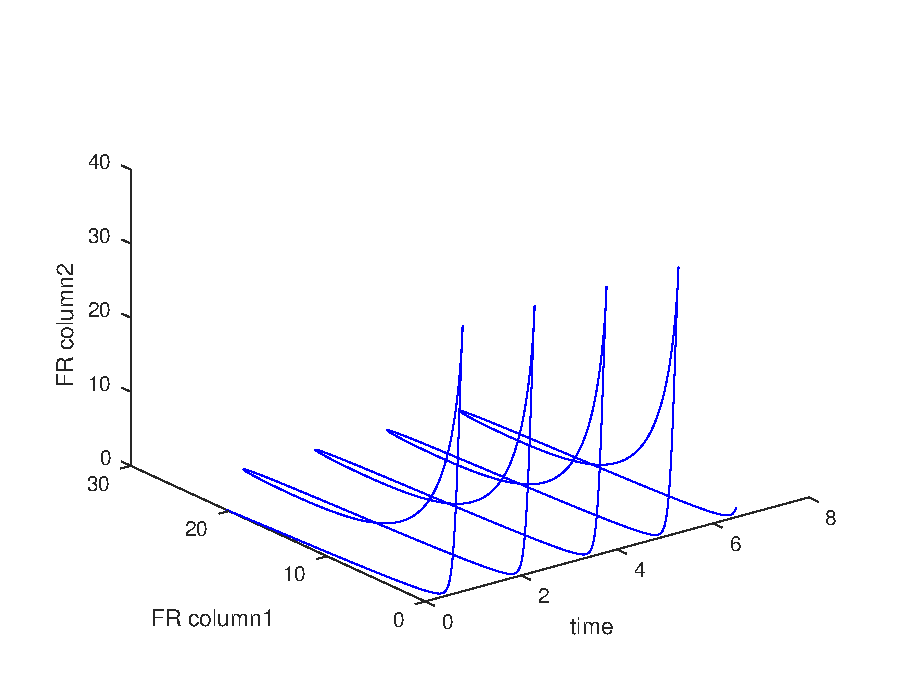
\includegraphics[width=\textwidth]{./images/FinalOralPlots/SyntheticOralPaper/SimFiringRate-with-Time.eps}
            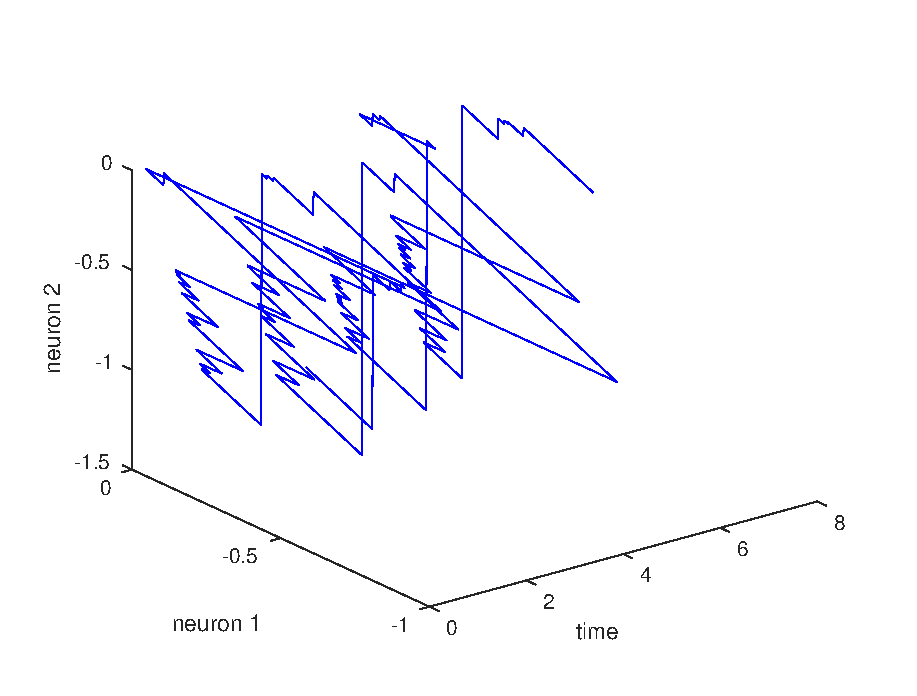
\includegraphics[width=\textwidth]{./images/SimPrevtime_with_time.eps}
            \caption[]%
            {{\small Simulated previous time data (Prevtime)}}  
            %{{\small Simulated firing rate data (FR)}}    
            \label{fig:Sim animal position in 3D}
        \end{subfigure}
        \caption[]%
         {\small  (a) Example of the firing rate of two neurons showing the modulation of the firing rates as the rat completes four and a half laps around a simulated circular track.
         (b) Example of the previous time of two neurons obtained after preprocessing  simulated spike times using  the 
         previous time measure. The pattern produced by the previous time measure is not clear in such a plot.} 
         \label{fig:Simulated_datasets}
\end{figure}
        
        
        
        
        \begin{figure}[H]
       \centering
        \begin{subfigure}[b]{0.475\textwidth}   
            \centering 
            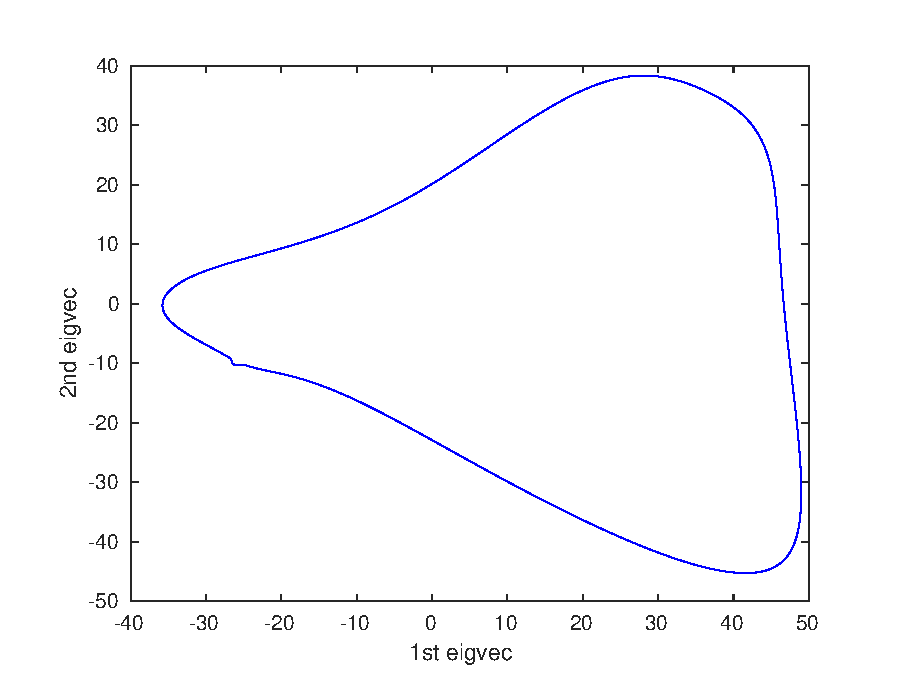
\includegraphics[width=\textwidth]{./images/FinalOralPlots/SyntheticOralPaper/SimFRPCA.eps}
           % 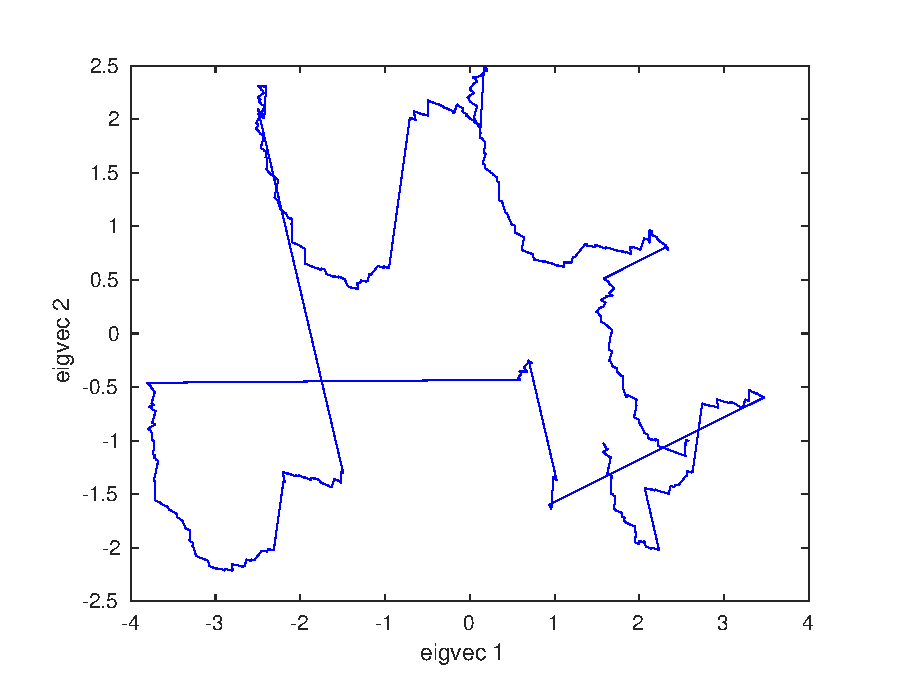
\includegraphics[width=\textwidth]{./images/FinalOralPlots/SyntheticOralPaper/SimPrevtimePCA.eps}
            \caption[]%
             {{\small PCA on FR}}   
            %{{\small PCA on Prevtime}}    
            \label{fig:PCA on Prevtime in 3D}
        \end{subfigure}
        \quad
        \begin{subfigure}[b]{0.475\textwidth}   
            \centering 
            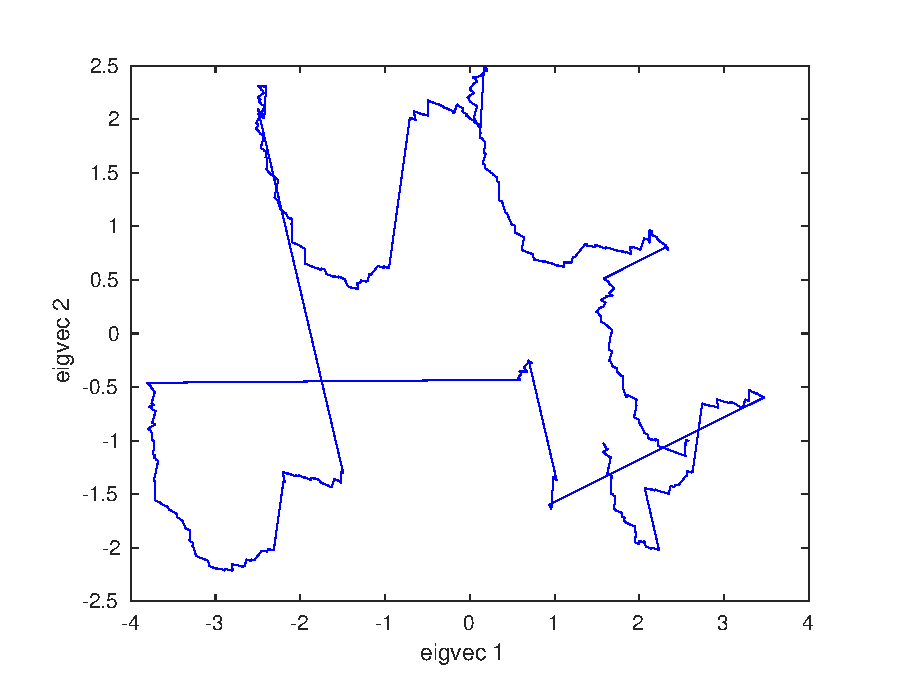
\includegraphics[width=\textwidth]{./images/FinalOralPlots/SyntheticOralPaper/SimPrevtimePCA.eps}
           % 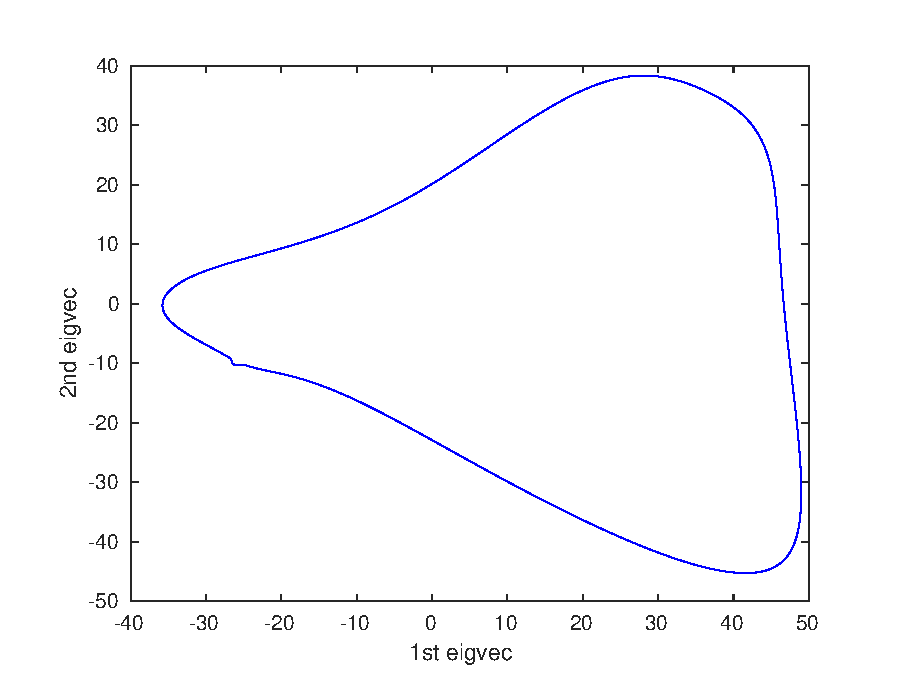
\includegraphics[width=\textwidth]{./images/FinalOralPlots/SyntheticOralPaper/SimFRPCA.eps}
            \caption[]%
             {{\small PCA on Prevtime}}   
           % {{\small PCA on FR}}    
            \label{fig:PCA on prevtime in 2D }
        \end{subfigure}
        \vskip\baselineskip
        \begin{subfigure}[b]{0.475\textwidth}   
            \centering 
             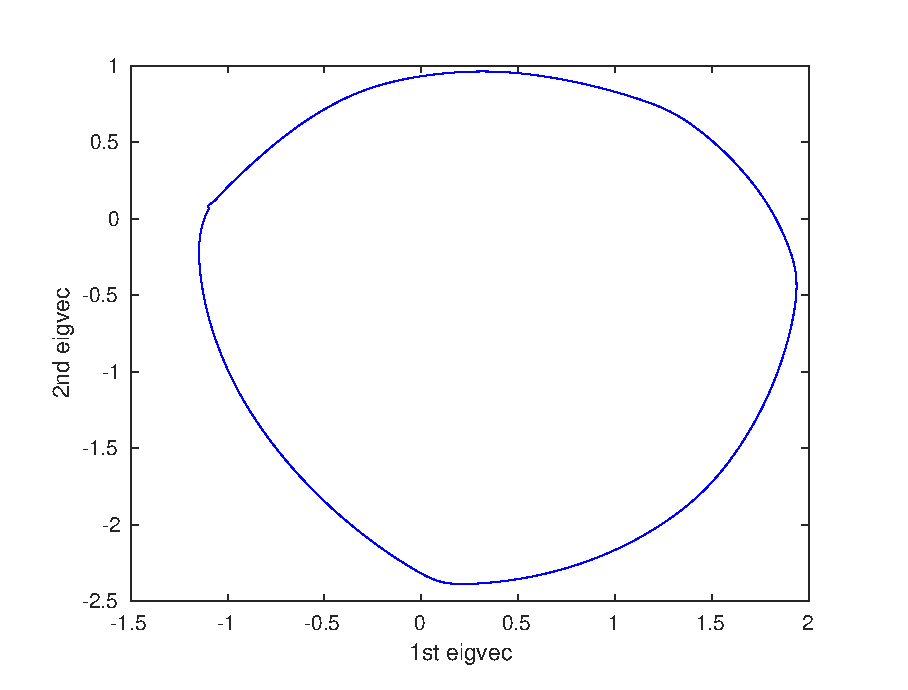
\includegraphics[width=\textwidth]{./images/FinalOralPlots/SyntheticOralPaper/SimFRDML1.eps}
          %  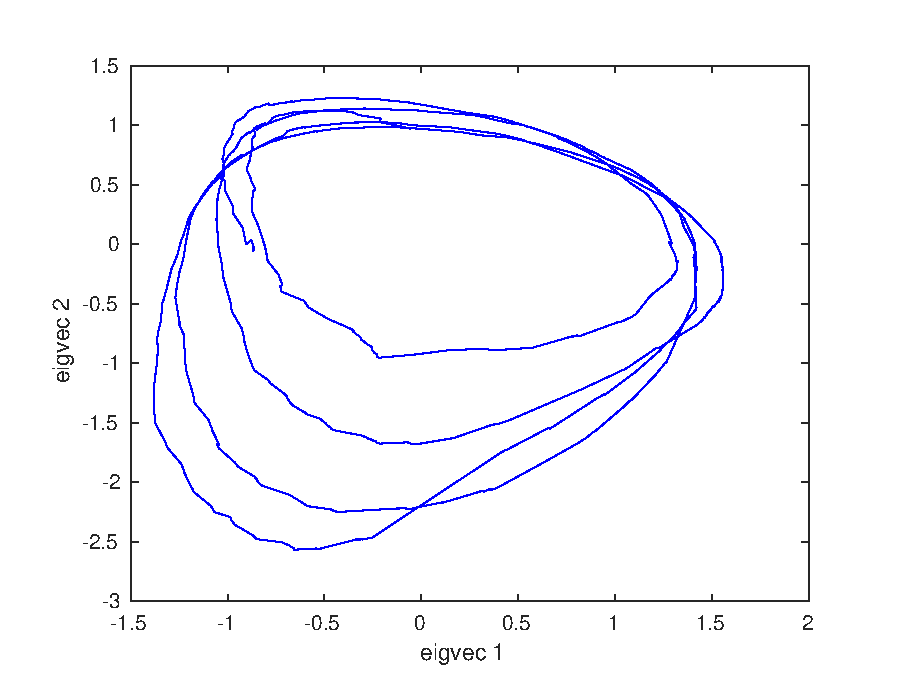
\includegraphics[width=\textwidth]{./images/FinalOralPlots/SyntheticOralPaper/SimPrevtimeDML1.eps}
            \caption[]%
             {{\small Diffusion Maps on FR}}    
            %{{\small Diffusion Maps on Prevtime}}    
            \label{fig:Diffusion maps on Prevtime in 3D}
        \end{subfigure}
        \quad
        \begin{subfigure}[b]{0.475\textwidth}   
            \centering 
             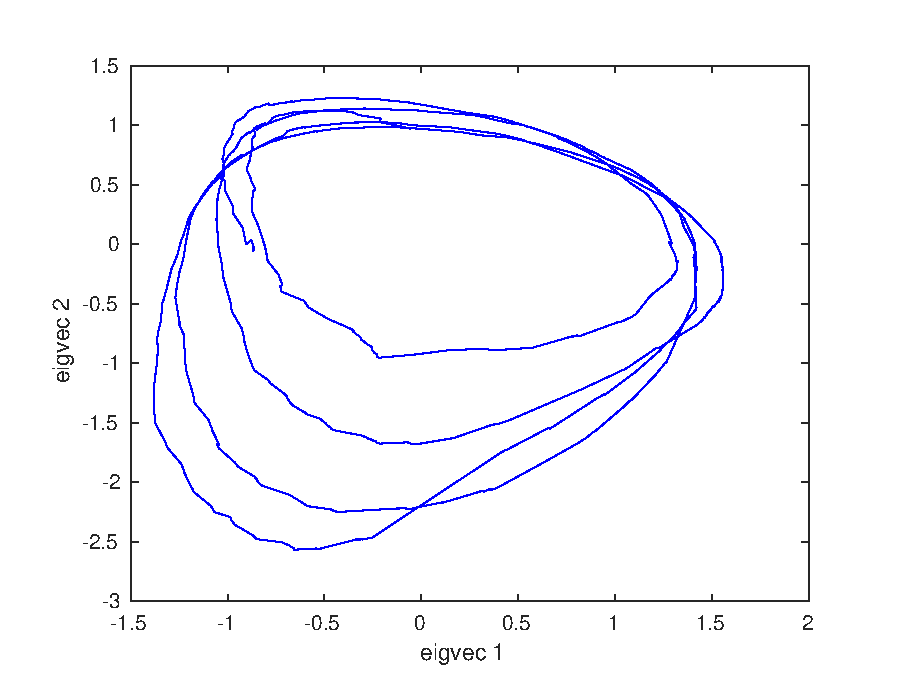
\includegraphics[width=\textwidth]{./images/FinalOralPlots/SyntheticOralPaper/SimPrevtimeDML1.eps}
           % 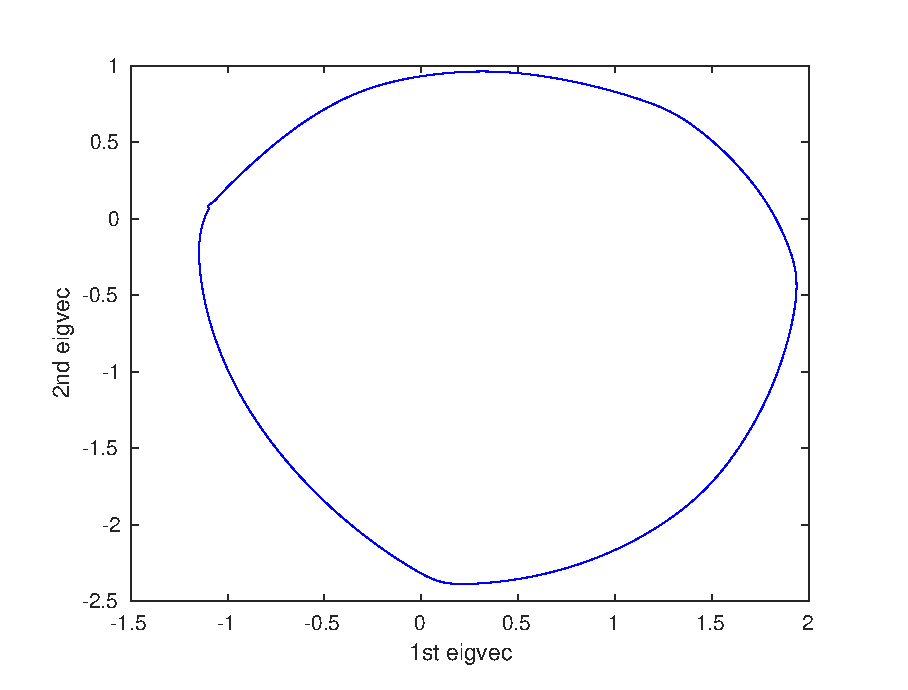
\includegraphics[width=\textwidth]{./images/FinalOralPlots/SyntheticOralPaper/SimFRDML1.eps}
            \caption[]%
            {{\small Diffusion Maps on Prevtime}}  
           % {{\small Diffusion Maps on FR}}    
            \label{fig:Diffusion maps on Prevtime in 3D }
        \end{subfigure}
        \caption[]%
         {\small Performance of PCA (first row) and Diffusion maps (second row) on simulated firing rate data (figure \ref{fig:Simulated_datasets}, left column)  and  previous  time data (figure \ref{fig:Simulated_datasets}, right column).
 A single point on any curve  represents the value of the first and second eigen vector at any time t.
(a, c) Each circle  corresponds to the four and a half laps made by the rat as the animal goes around a circular track. All the laps are superimposed on top of each other because the results in the left column are obtained after applying PCA  and Diffusion maps on clean firing rate data (with no noise). 
(b) Example showing that PCA applied to previous time data fails to reveal the four and a half laps taken by the rat around a circular track. 
(d)  Example showing that  Diffusion maps applied to previous time data recovers the four and a half laps taken by the rat around the circular  track. Since the rat's position in space is a circular curve parametrized in time, the top
         two eigen vectors of diffusion maps on previous time data capture the circular motion of the rat.} 
        \label{fig:DiffMaps_PCA_on_Prevtime_FR}
\end{figure}



















%\newpage

%%%%%%%%%%%%%%%%%%%%  Firing rate %%%%%%%%%%%%%%%%%%%%%%%%%%%%%%%%%%%%%%%%%%%%%%%%%%


%\begin{figure}[H]
%        \centering
%        \begin{subfigure}[b]{0.475\textwidth}
%            \centering
%            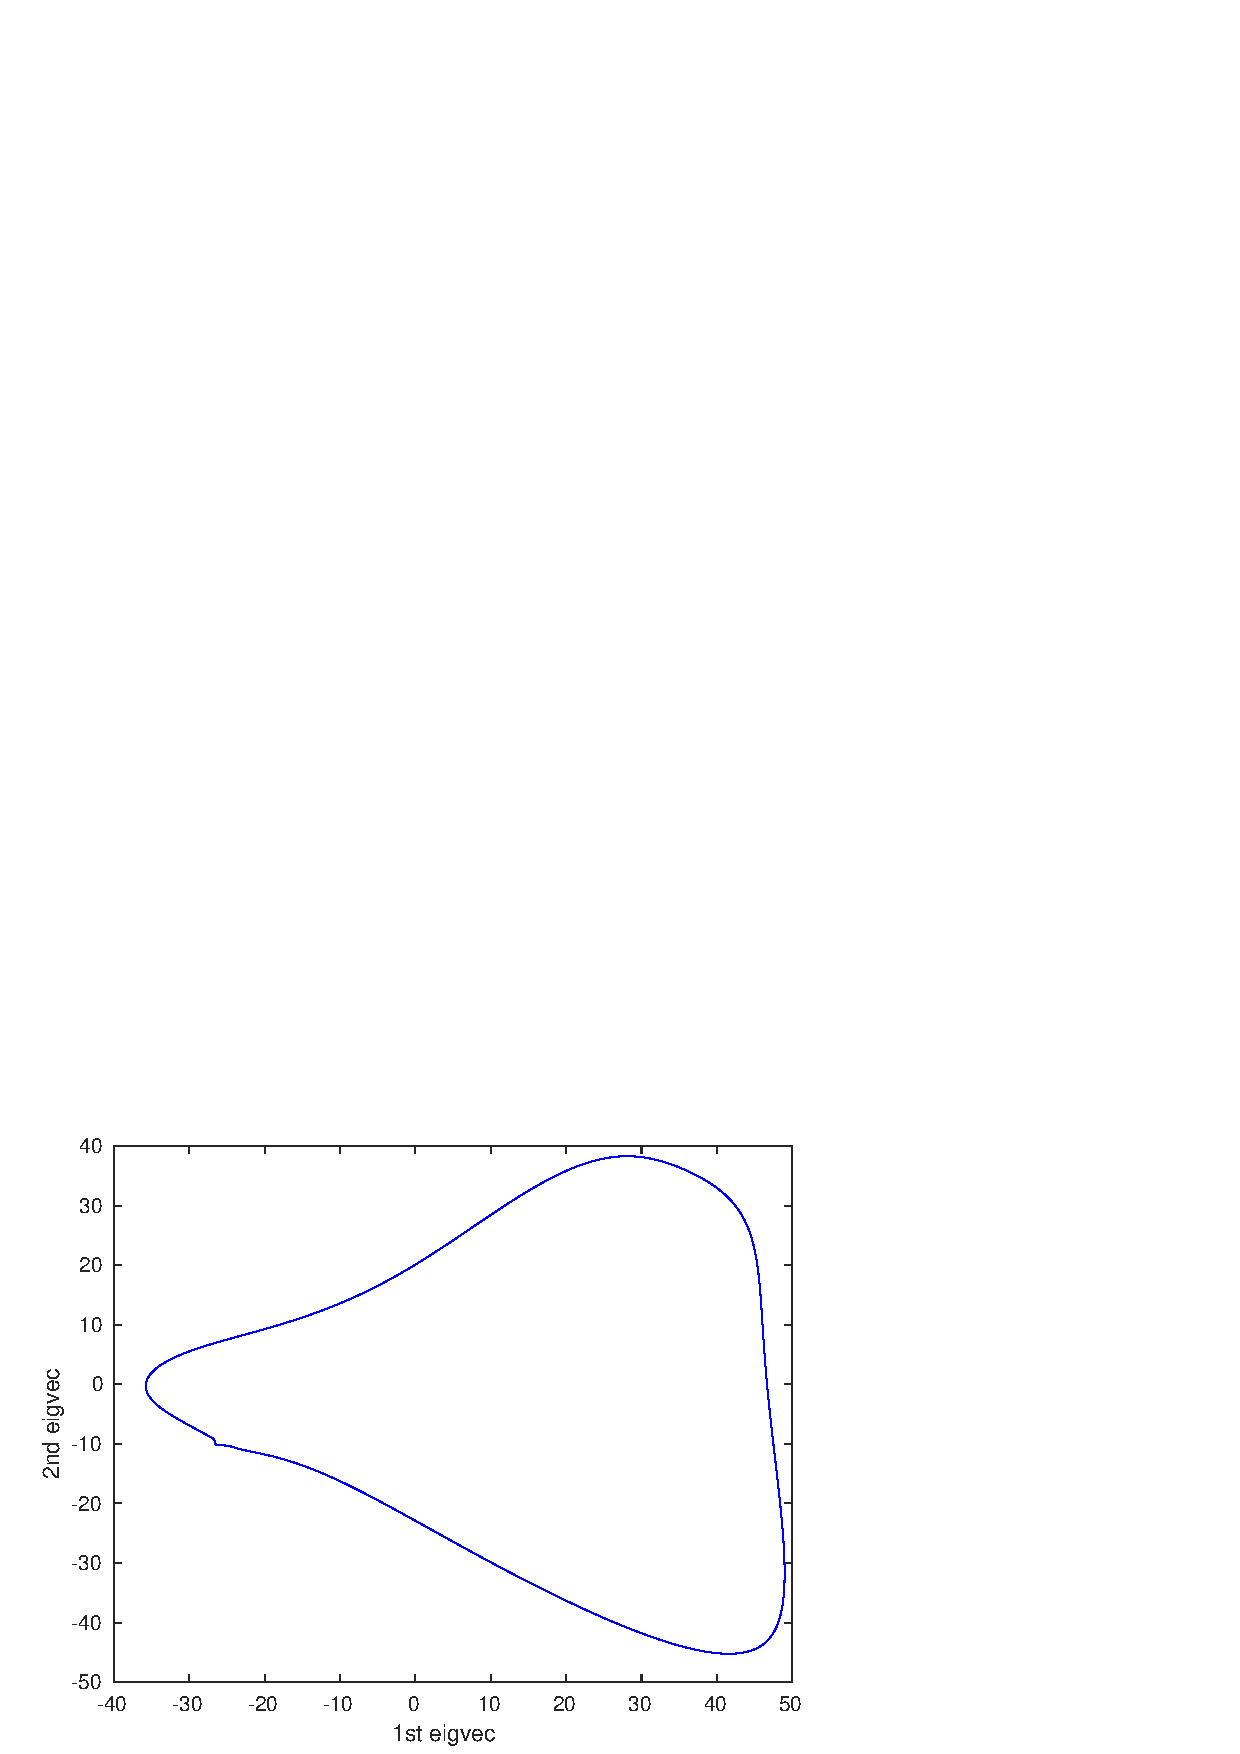
\includegraphics[width=\textwidth]{./images/FinalOralPlots/SyntheticOralPaper/SimFRPCA.pdf}
%            \caption[PCA on FR]%
%            {{\small PCA on FR}}    
%            \label{fig:PCA on FR in 3D}
%        \end{subfigure}
%        \hfill
%        \begin{subfigure}[b]{0.475\textwidth}  
%            \centering 
%            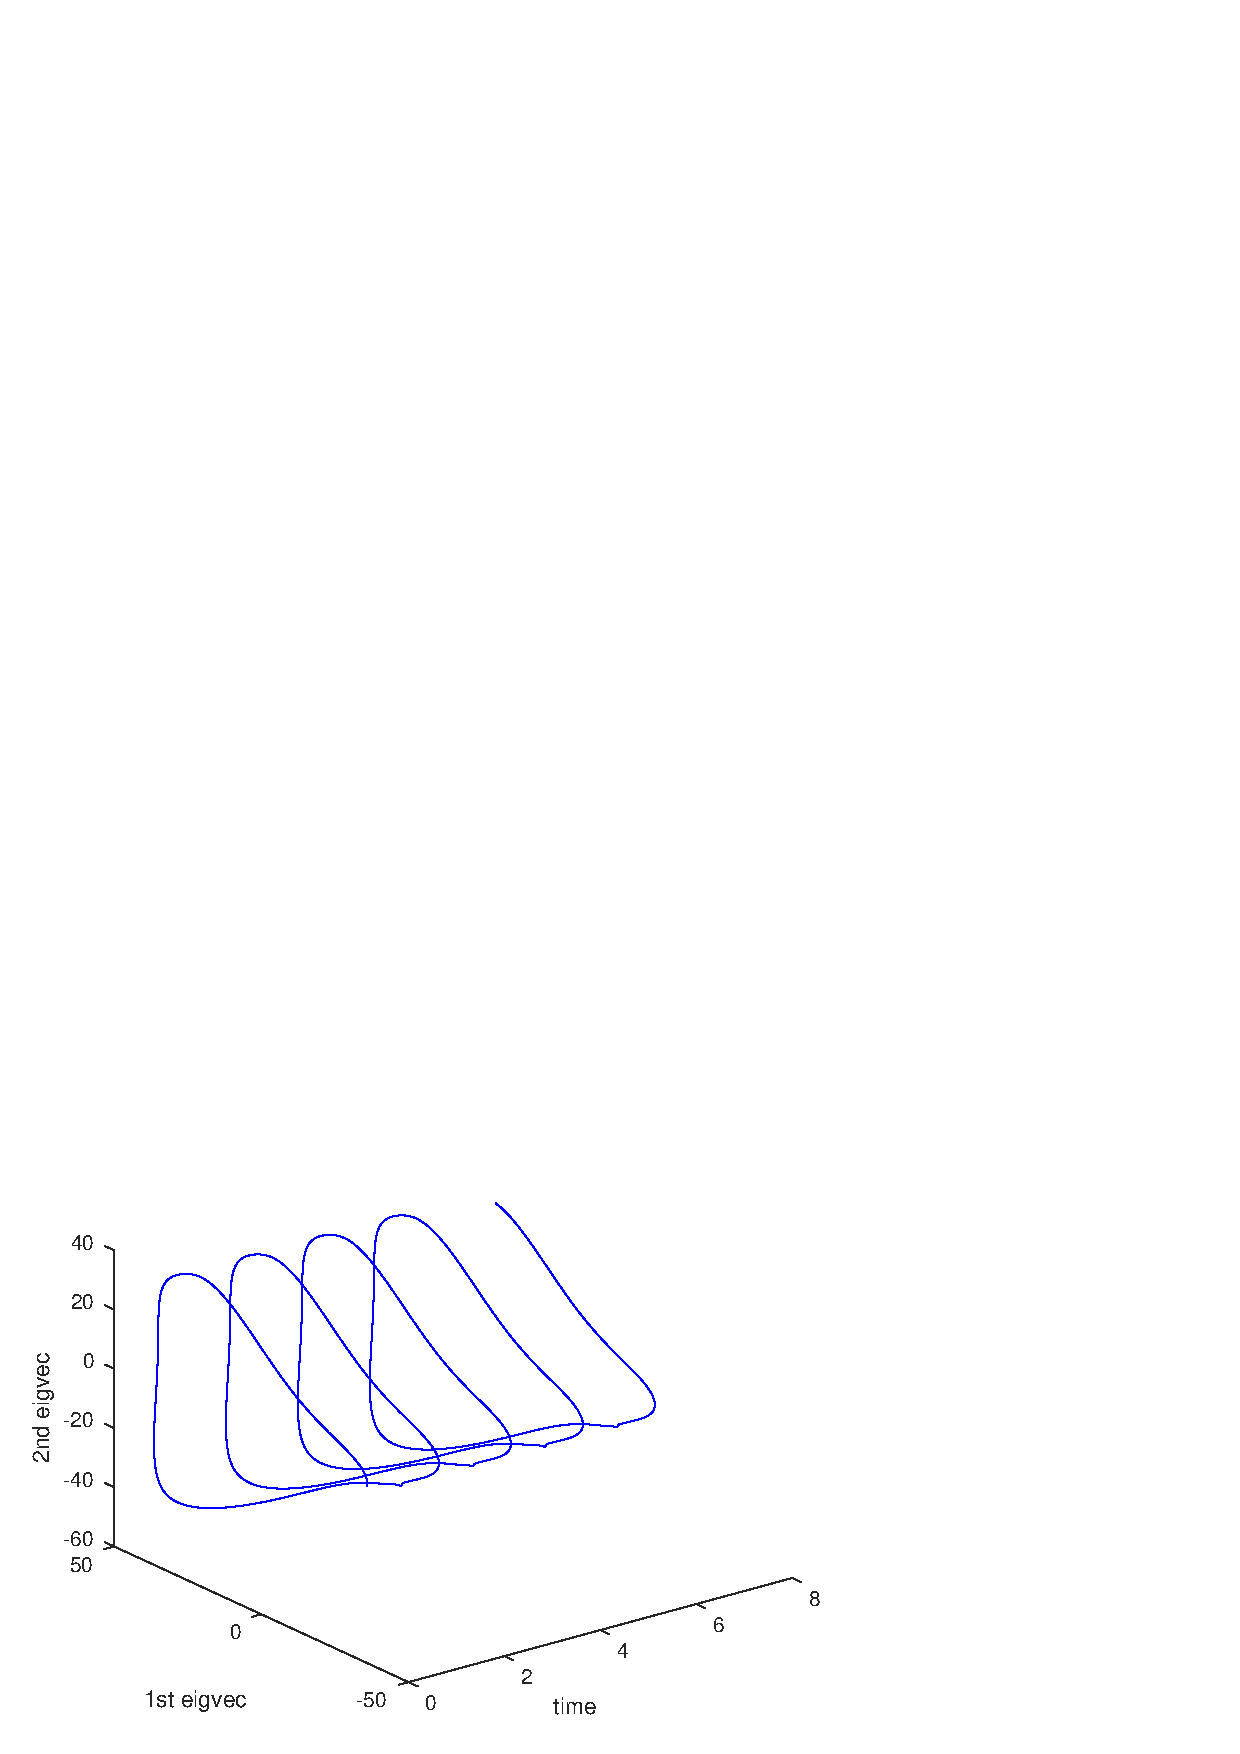
\includegraphics[width=\textwidth]{./images/FinalOralPlots/SyntheticOralPaper/SimFRPCA-with-time.pdf}
%            \caption[]%
%            {{\small PCA on FR}}    
%            \label{fig:PCA on FR in 2D}
%        \end{subfigure}
%        \vskip\baselineskip
%        \begin{subfigure}[b]{0.475\textwidth}   
%            \centering 
%            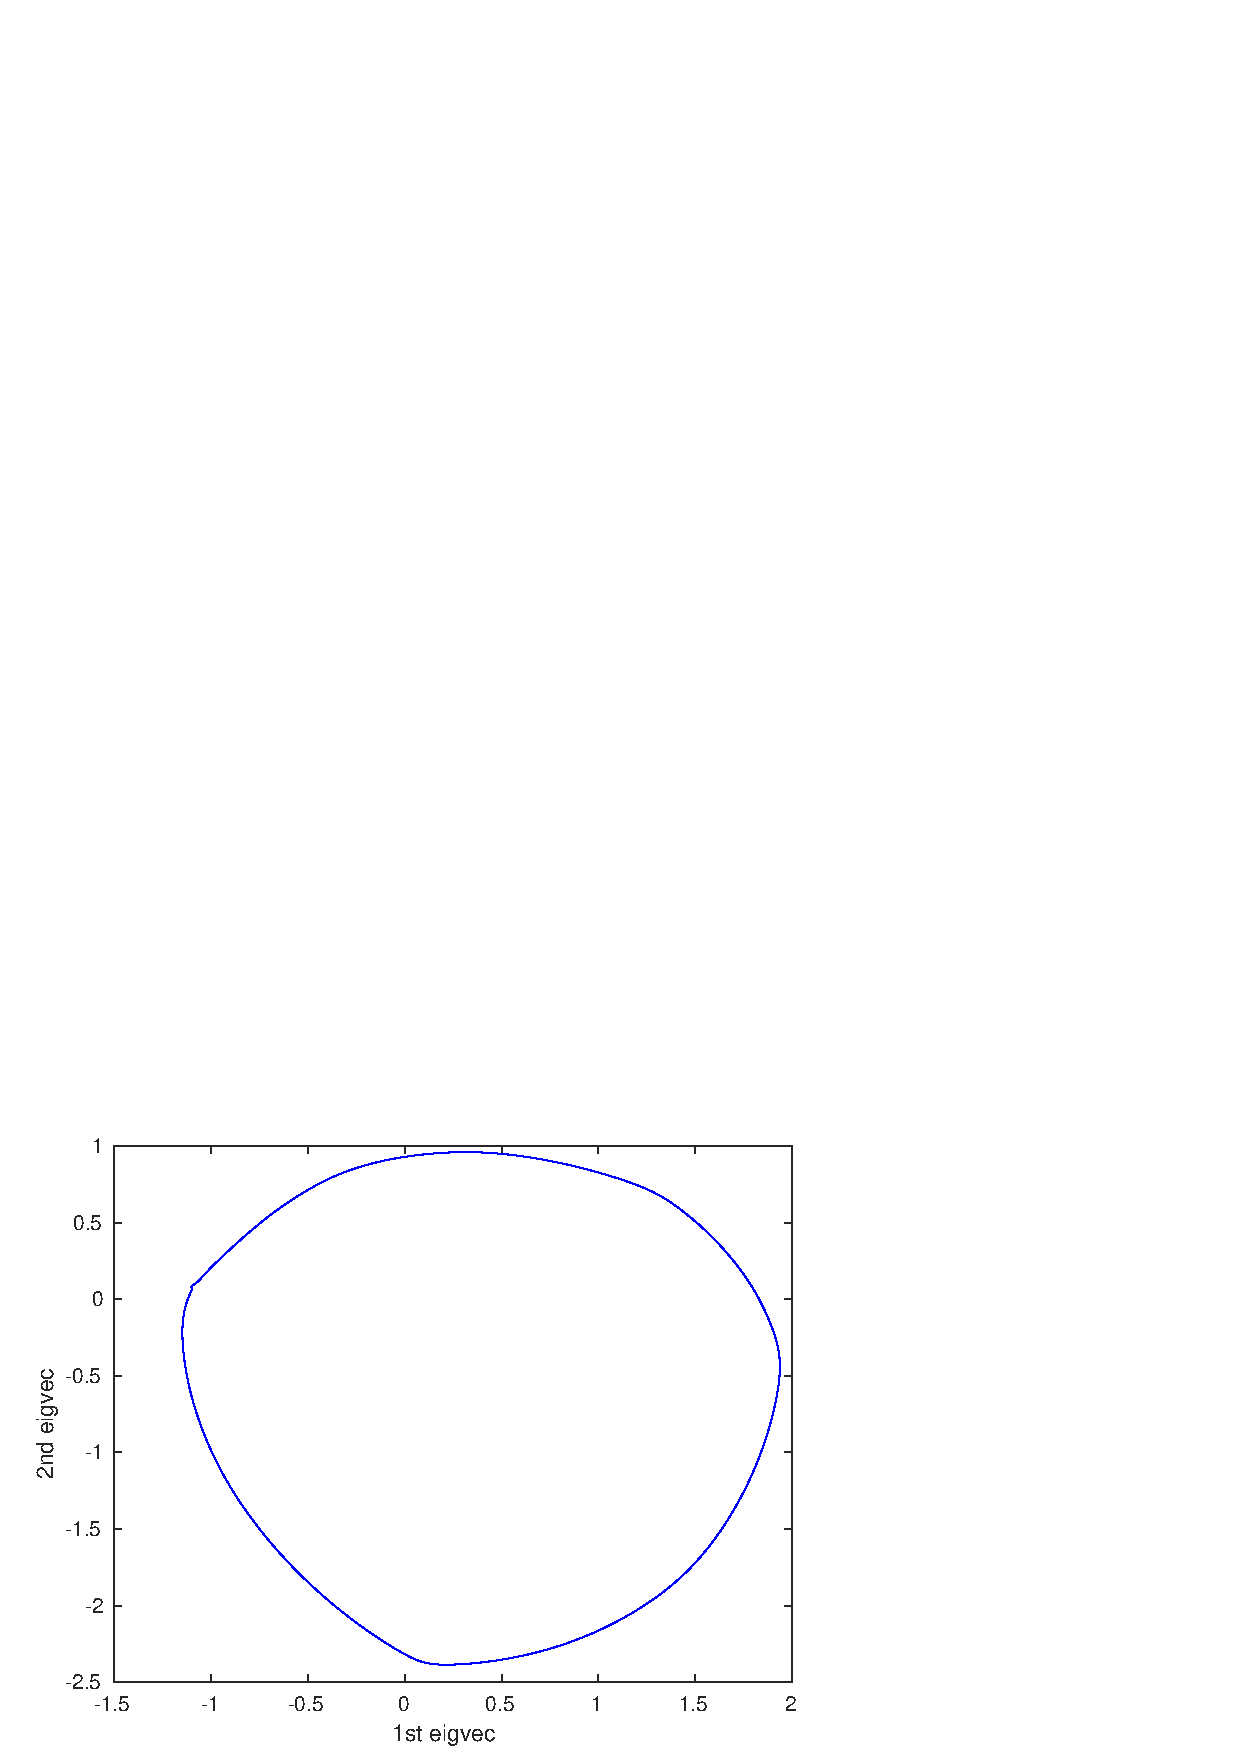
\includegraphics[width=\textwidth]{./images/FinalOralPlots/SyntheticOralPaper/SimFRDML1.pdf}
%            \caption[]%
%            {{\small Diffusion Maps on FR}}    
%            \label{fig:Diffusion maps on FR in 3D}
%        \end{subfigure}
%        \quad
%        \begin{subfigure}[b]{0.475\textwidth}   
%            \centering 
%            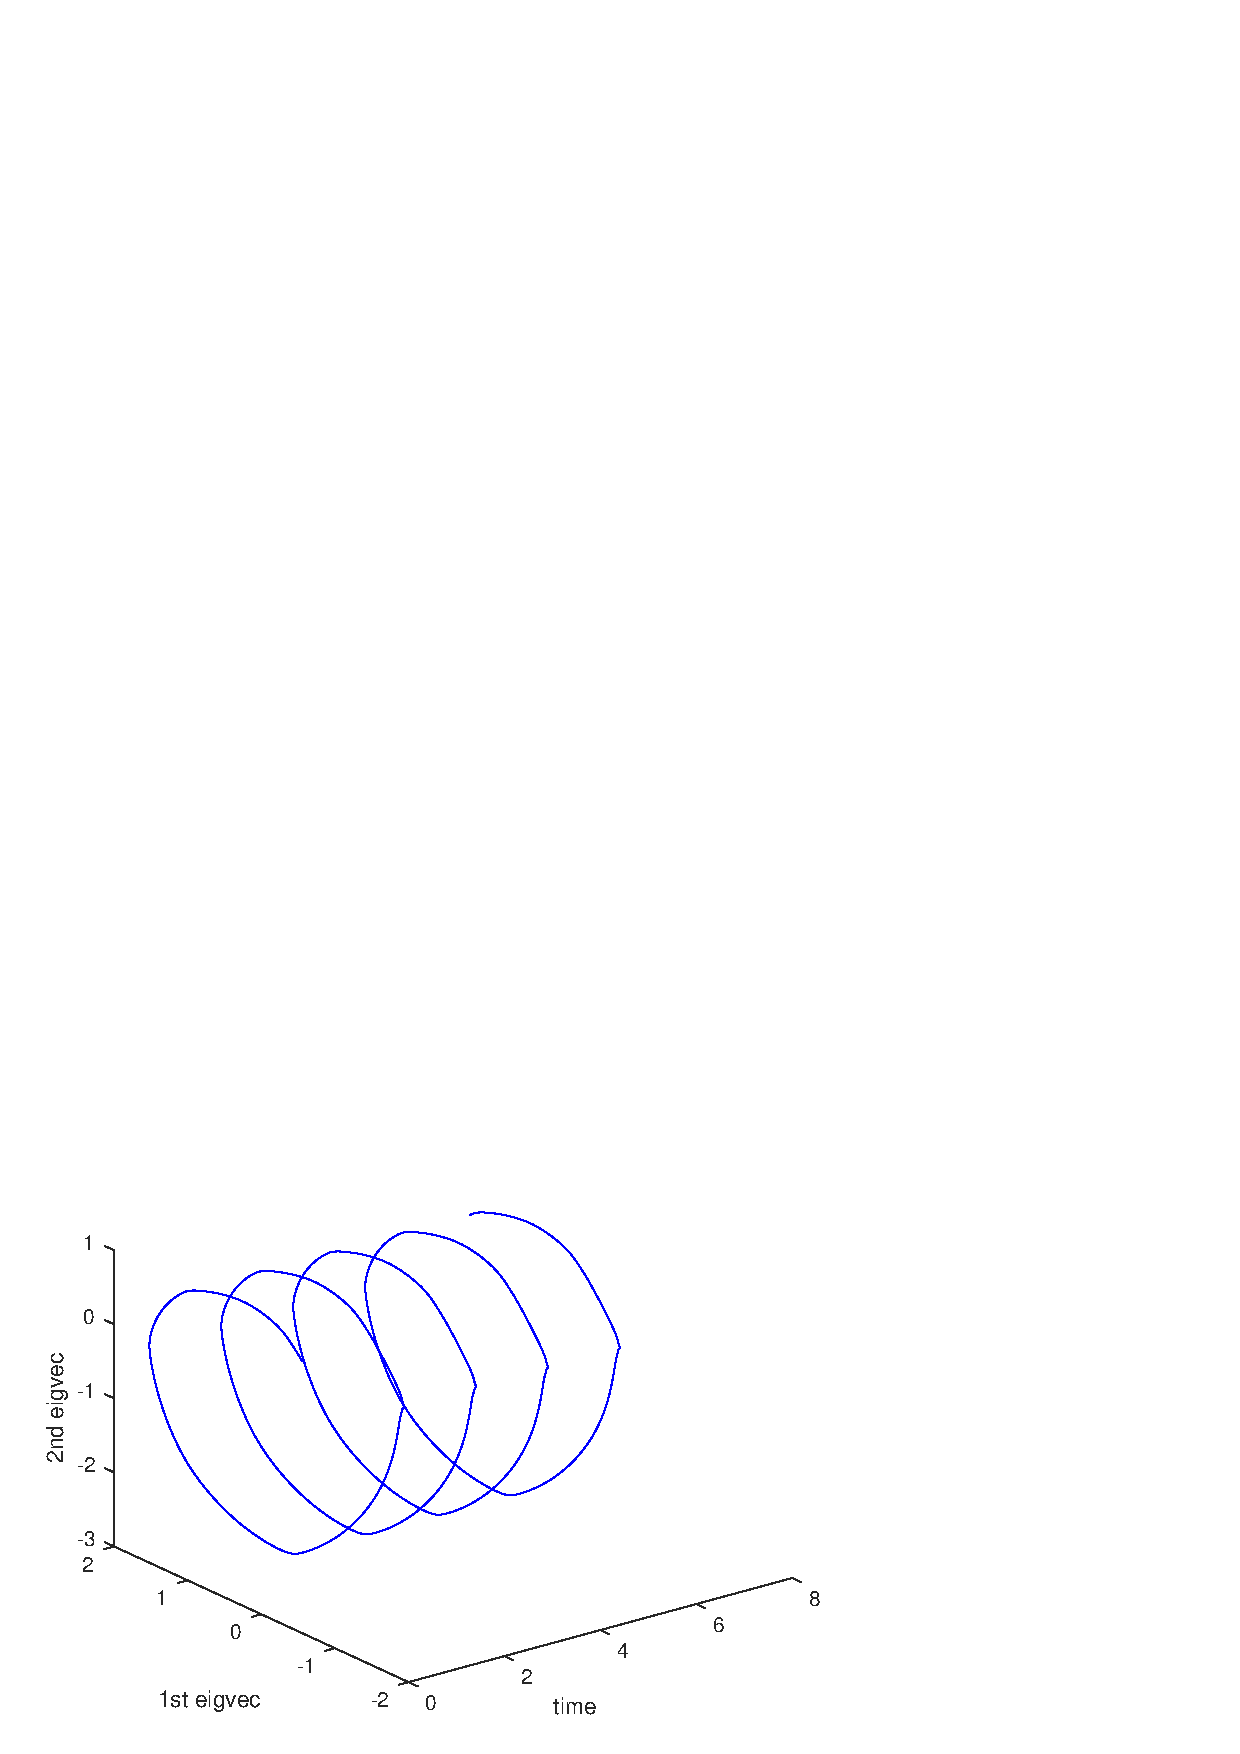
\includegraphics[width=\textwidth]{./images/FinalOralPlots/SyntheticOralPaper/SimFRDML1-with-time.pdf}
%            \caption[]%
%            {{\small Diffusion Maps on FR}}    
%            \label{fig:Diffusion maps on FR in 2D }
%        \end{subfigure}
%        \caption[small Performance of Diffusion maps and PCA on simulated firing rate data ]
%        {\small Performance of Diffusion maps and PCA on simulated firing rate data} 
%        \label{fig:DiffMaps_PCA_on_FR}
%    \end{figure}
%
%


%Next, we show the results of diffusion maps with $l_{1}$ distance 
%and PCA on simulated previous time data (Prevtime). 

%%%%%%%%%%%%%%%%%%%%%%%%%%%% Prevtime and simulated position %%%%%%%%%%%%%%%%%%%%%%%%%%%%%

%\begin{figure}[H]
%        \centering
%        \begin{subfigure}[b]{0.475\textwidth}
%            \centering
%            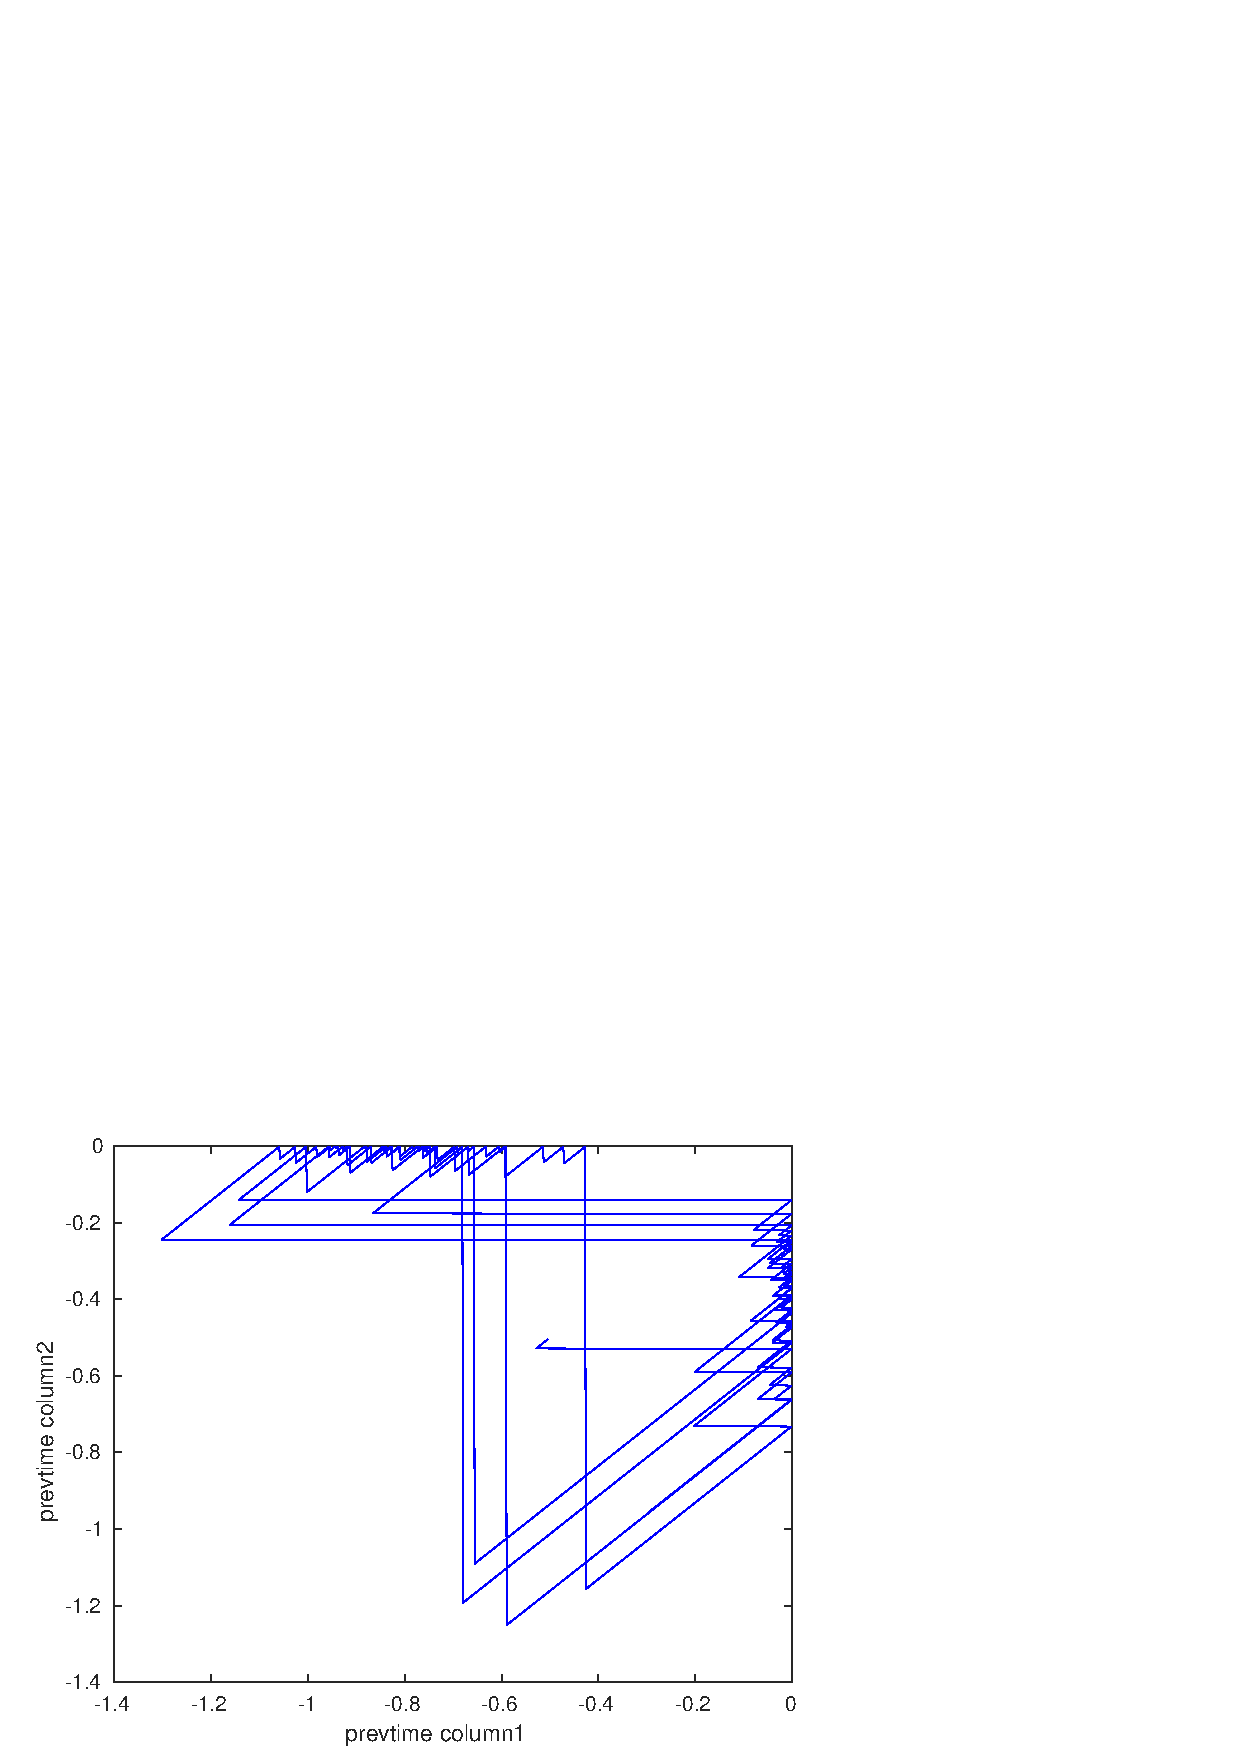
\includegraphics[width=\textwidth]{./images/FinalOralPlots/SyntheticOralPaper/SimPrevtime.pdf}
%            \caption[Simulated Prevtime]%
%            {{\small Simulated Prevtime}}    
%            \label{fig:Prevtime in 3D}
%        \end{subfigure}
%        \hfill
%        \begin{subfigure}[b]{0.475\textwidth}  
%            \centering 
%            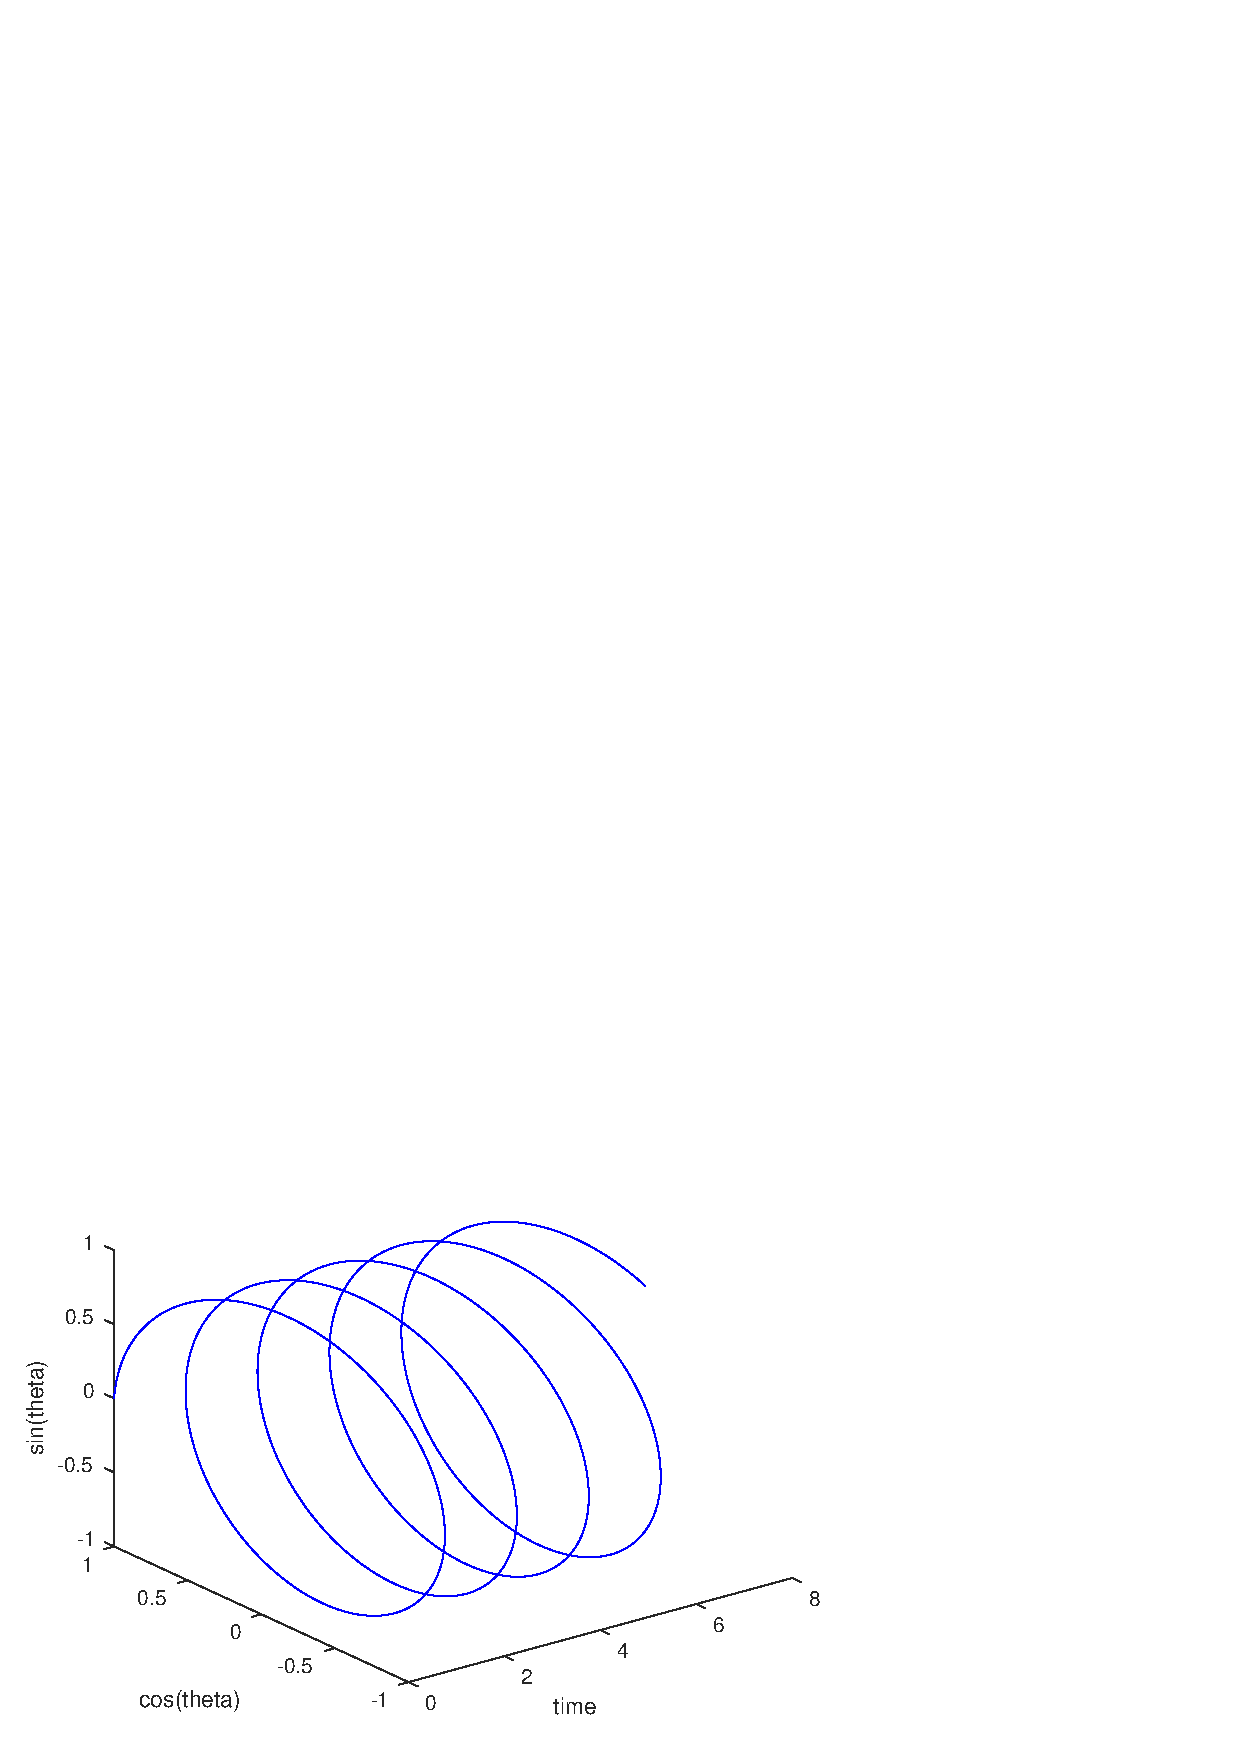
\includegraphics[width=\textwidth]{./images/FinalOralPlots/SyntheticOralPaper/SimRatPosition.pdf}
%            \caption[]%
%            {{\small Simulated animal position}}    
%            \label{fig:Sim animal position in 3D}
%        \end{subfigure}
%        \vskip\baselineskip
%        \begin{subfigure}[b]{0.475\textwidth}   
%            \centering 
%            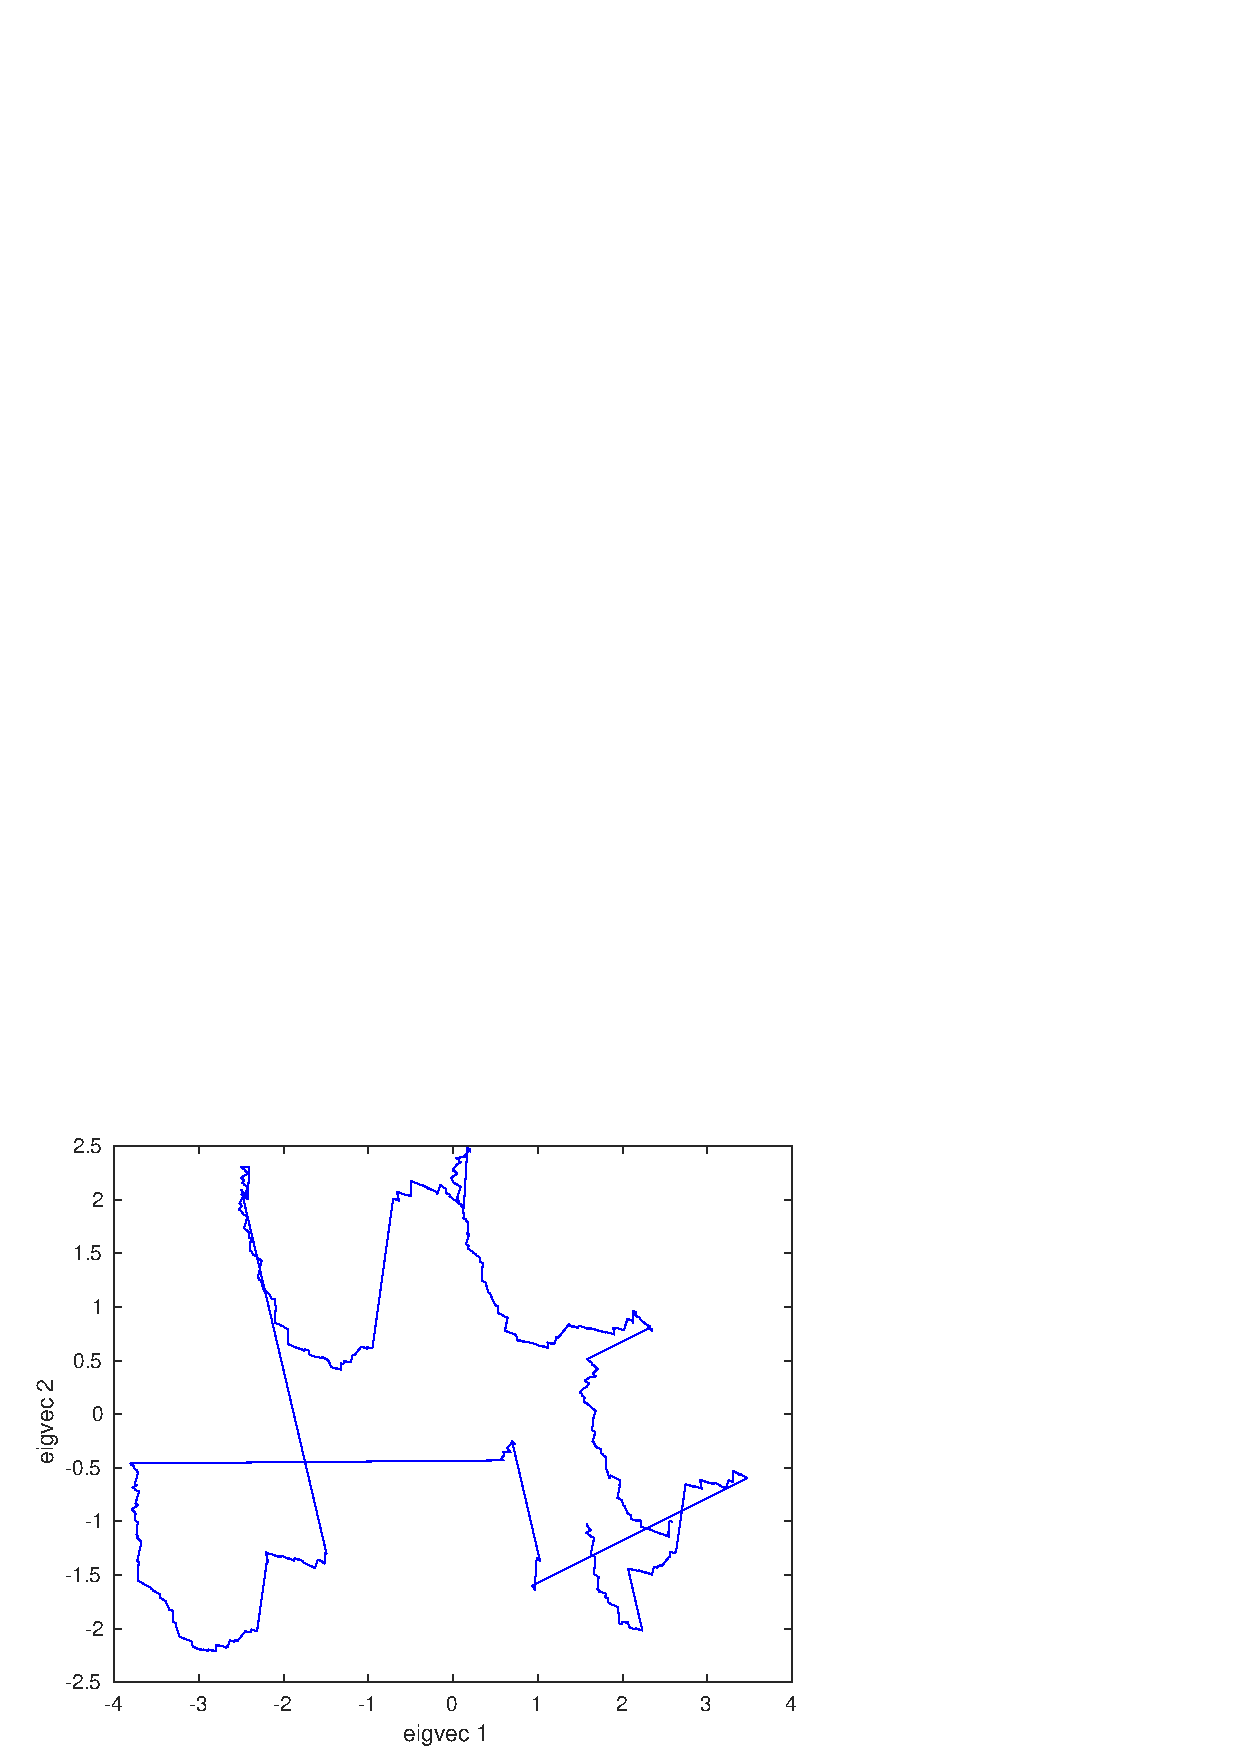
\includegraphics[width=\textwidth]{./images/FinalOralPlots/SyntheticOralPaper/SimPrevtimePCA.pdf}
%            \caption[]%
%            {{\small PCA on Prevtime}}    
%            \label{fig:PCA on Prevtime in 3D}
%        \end{subfigure}
%        \quad
%        \begin{subfigure}[b]{0.475\textwidth}   
%            \centering 
%            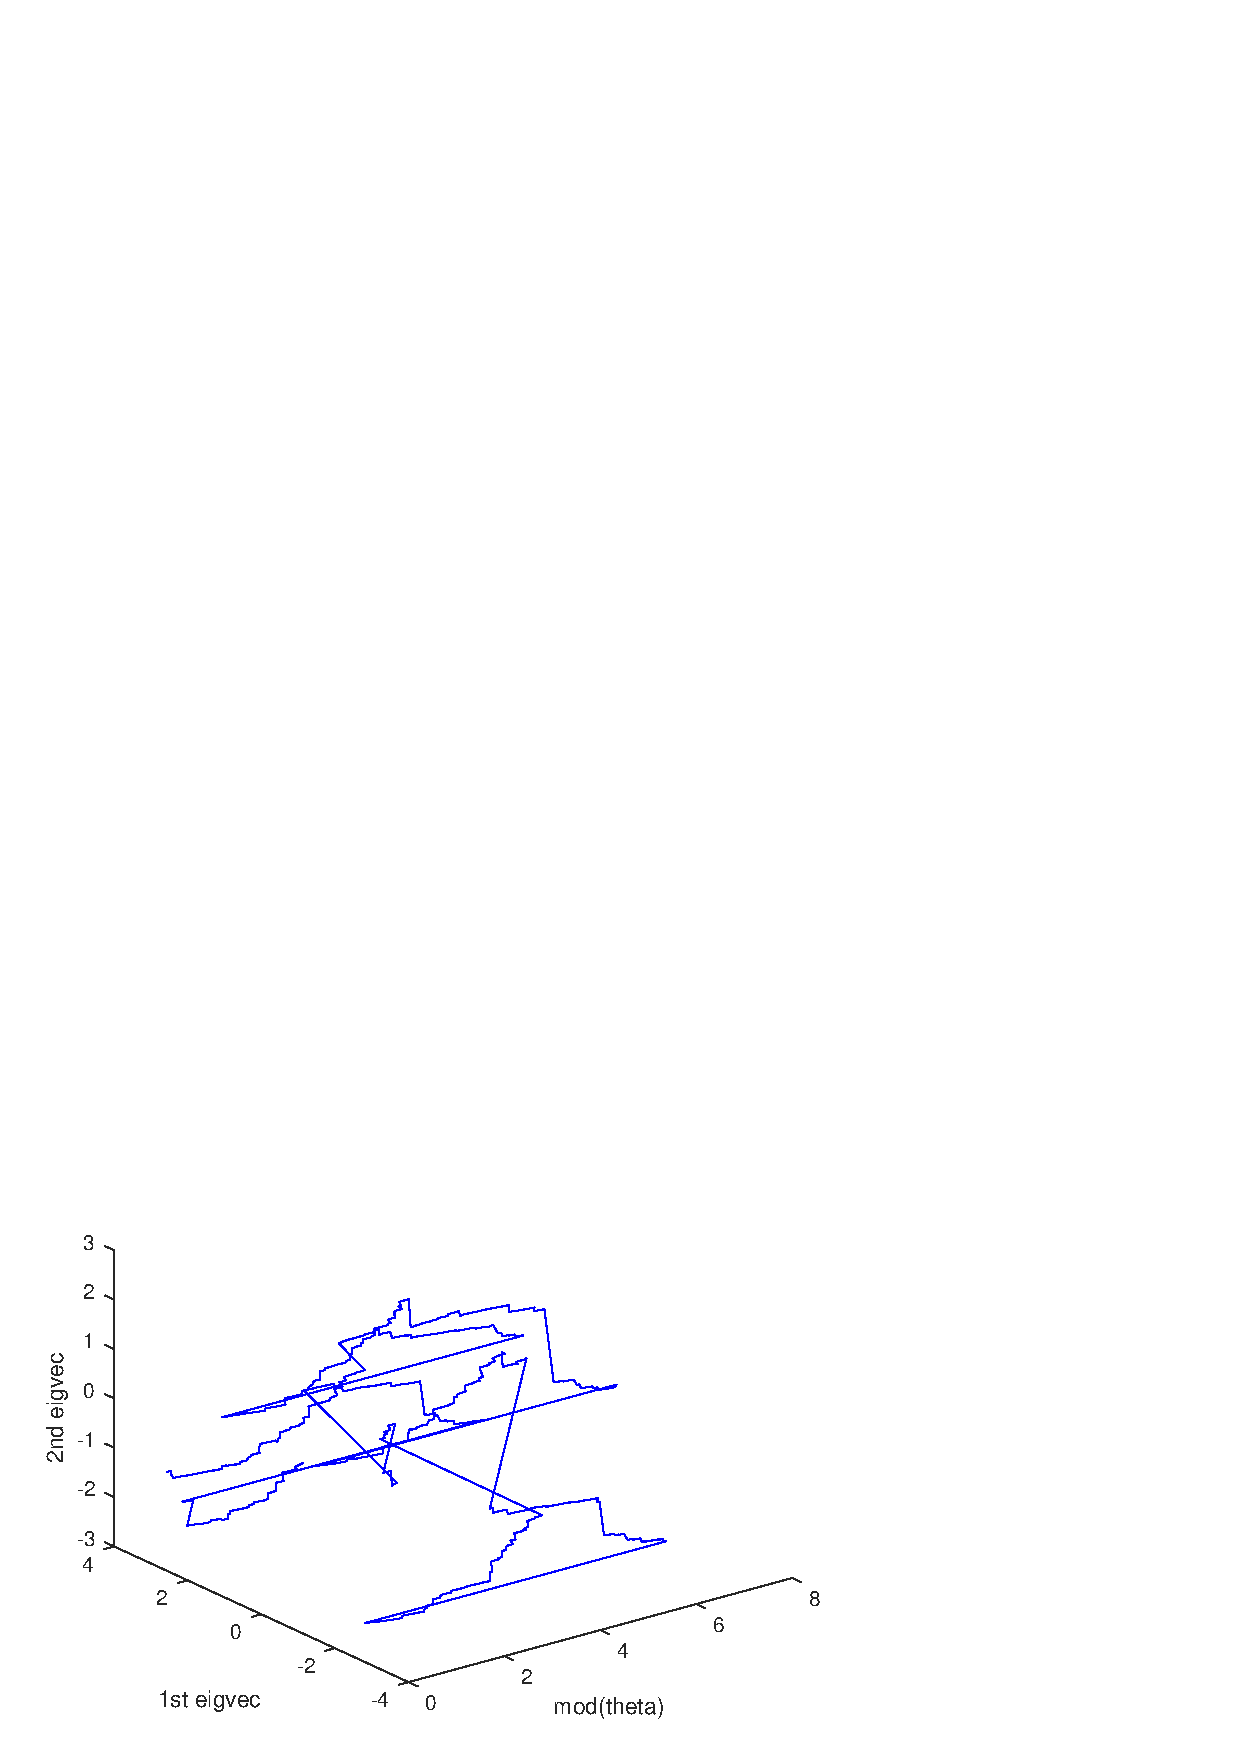
\includegraphics[width=\textwidth]{./images/FinalOralPlots/SyntheticOralPaper/SimPrevtimePCA-with-Position.pdf}
%            \caption[]%
%            {{\small PCA on prevtime}}    
%            \label{fig:PCA on prevtime in 2D }
%        \end{subfigure}
%        \vskip\baselineskip
%        \begin{subfigure}[b]{0.475\textwidth}   
%            \centering 
%            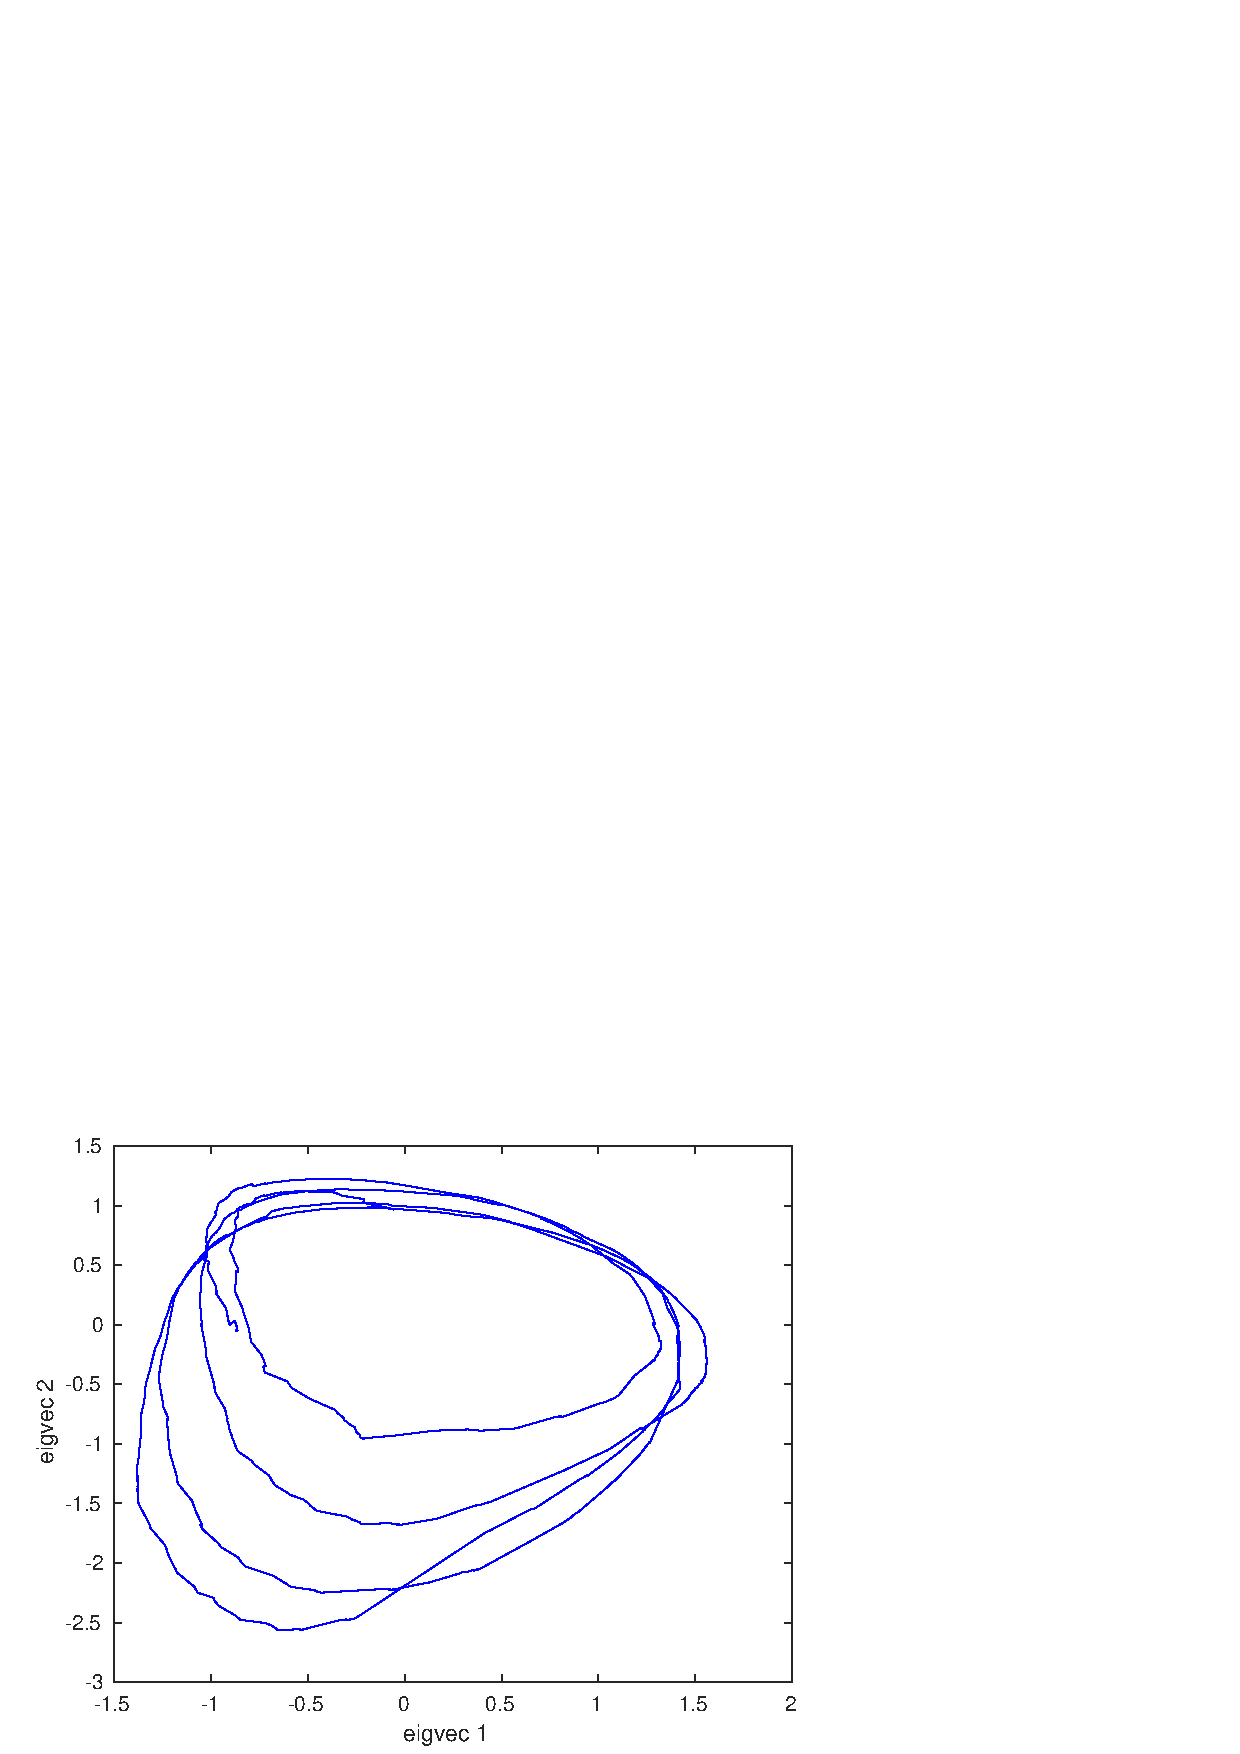
\includegraphics[width=\textwidth]{./images/FinalOralPlots/SyntheticOralPaper/SimPrevtimeDML1.pdf}
%            \caption[]%
%            {{\small Diffusion Maps on Prevtime}}    
%            \label{fig:Diffusion maps on Prevtime in 3D}
%        \end{subfigure}
%        \quad
%        \begin{subfigure}[b]{0.475\textwidth}   
%            \centering 
%            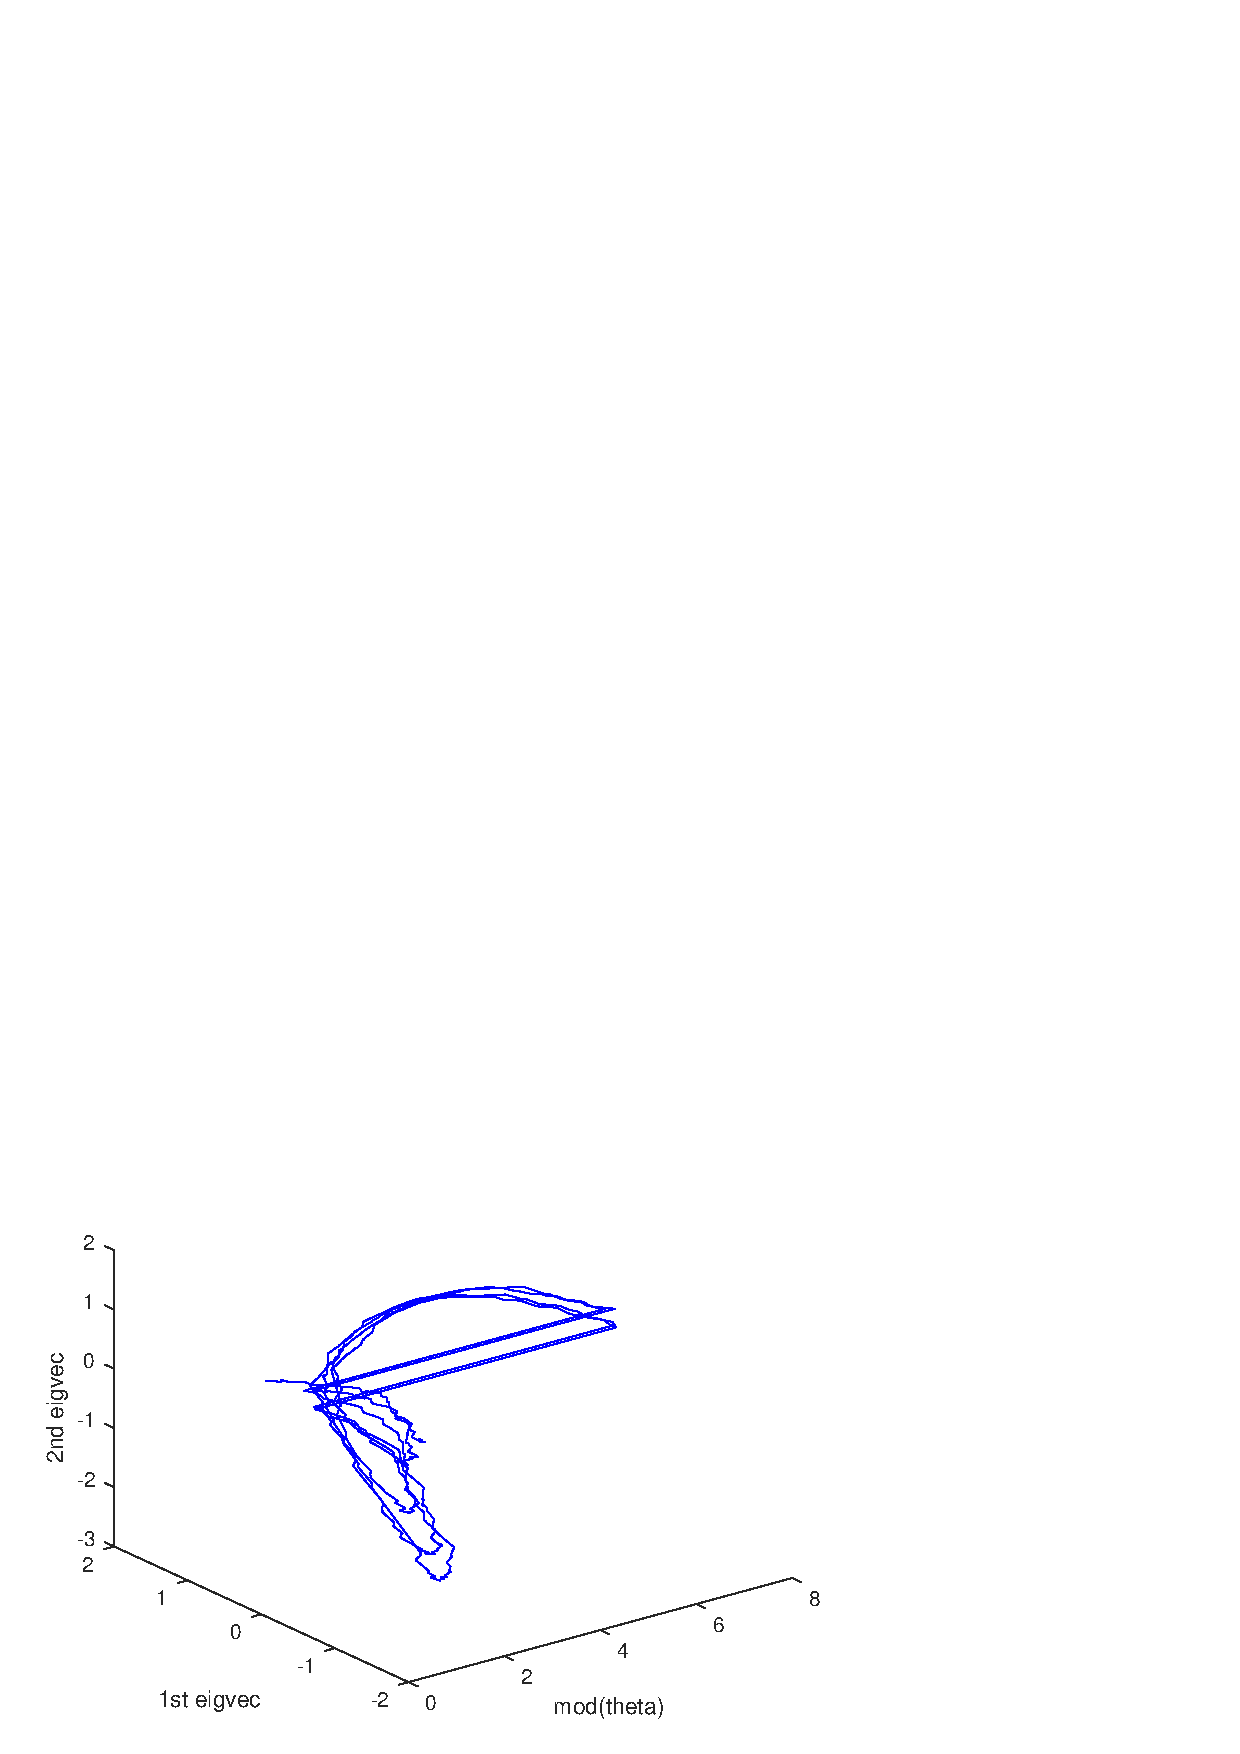
\includegraphics[width=\textwidth]{./images/FinalOralPlots/SyntheticOralPaper/SimPrevtimeDML1-with-Position.pdf}
%            \caption[]%
%            {{\small Diffusion Maps on Prevtime}}    
%            \label{fig:Diffusion maps on Prevtime in 3D }
%        \end{subfigure}
%        \caption[Performance of Diffusion maps and PCA on simulated previous time data ]
%        {\small Performance of Diffusion maps and PCA on simulated previous time data} 
%        \label{fig:DiffMaps_PCA_on_Prevtime}
%\end{figure}
%


















 































































%\begin{itemize}
%\item show the graphs/results package
%\item this is how we're interpreting the results
%\item why does this matter?
%\item what measure of goodness did you use?
%(Fisher Vs Shannon information)

%%==========suggested by Duane============================================
%\item Mention that there are other ways of checking measures of goodness
% e.g the one provided by diffusion maps, Bayesian decoding refer to the nature
% and review artcicle.


%\end{itemize}







